\newcommand{\DoNotLoadEpstopdf}{}
\documentclass[11pt]{article}
\usepackage[T1]{fontenc}
\usepackage{lmodern}
\usepackage[margin=1in]{geometry}
\usepackage{amsmath,amssymb,amsthm,mathtools}
\usepackage{microtype}
\usepackage{enumitem}
\usepackage{booktabs,array,flafter}
\usepackage{tikz}
\usetikzlibrary{arrows.meta,positioning}
\usepackage[numbers,sort&compress]{natbib}
\usepackage{hyperref}
\hypersetup{colorlinks=true,linkcolor=black,citecolor=black,urlcolor=blue,
  pdftitle={Fujita's freeness conjecture},pdfauthor={OpenAI}}
\pdfinfoomitdate=1
\pdftrailerid{}
\pdfsuppressptexinfo=15
\numberwithin{equation}{section}
\newtheorem{theorem}{Theorem}[section]
\newtheorem{proposition}[theorem]{Proposition}
\newtheorem{lemma}[theorem]{Lemma}
\newtheorem{corollary}[theorem]{Corollary}
\theoremstyle{definition}
\newtheorem{definition}[theorem]{Definition}
\theoremstyle{remark}
\newtheorem{remark}[theorem]{Remark}
\newcommand{\C}{\mathbb C}
\newcommand{\N}{\mathbb N}
\newcommand{\R}{\mathbb R}
\newcommand{\Q}{\mathbb Q}
\newcommand{\Z}{\mathbb Z}
\newcommand{\cO}{\mathcal O}
\newcommand{\A}{A}
\newcommand{\floor}[1]{\left\lfloor #1\right\rfloor}
\newcommand{\ceil}[1]{\left\lceil #1\right\rceil}
\DeclareMathOperator{\ord}{ord}
\DeclareMathOperator{\mult}{mult}
\DeclareMathOperator{\lct}{lct}
\DeclareMathOperator{\Supp}{Supp}
\DeclareMathOperator{\conv}{conv}
\DeclareMathOperator{\Bl}{Bl}
\DeclareMathOperator{\codim}{codim}
\DeclareMathOperator{\im}{im}
\DeclareMathOperator{\cent}{cent}
\DeclareMathOperator{\divisor}{div}
\setlist{nosep}
\setlength{\emergencystretch}{1.5em}

\title{Fujita's freeness conjecture}
\author{OpenAI}
\date{September 23, 2026}

\begin{document}
\maketitle
\begin{abstract}
We prove Fujita's freeness conjecture. If $X$ is a smooth complex
projective variety of dimension $n$ and $L$ is an ample line bundle,
then $K_X+mL$ is globally generated for every integer $m\geq n+1$.
\end{abstract}

\section{Introduction}
We use additive notation for line bundles. Fujita's freeness conjecture
\cite{fujita1987}
predicts that the canonical bundle becomes globally generated after
twisting by $n+1$ copies of an arbitrary ample line bundle on a smooth
projective $n$-fold. The ample bundle itself need not have any nonzero
sections. We prove the following precise form.

\begin{theorem}\label{thm:main}
Let $X$ be a smooth connected projective variety over $\C$ of dimension
$n\geq 1$, and let $L$ be an ample line bundle on $X$. Then
\[
                    K_X+(n+1)L
\]
is generated by its global sections.
\end{theorem}

The connectedness assumption only fixes notation: the assertion applies
to each connected component. In dimension zero every line bundle is
globally generated.

The exponent is sharp: for $X=\mathbb P^n$ and $L=\cO_{\mathbb P^n}(1)$,
the bundle $K_X+(n+1)L$ is trivial, whereas $K_X+nL$ has no nonzero
sections. Global generation asks for a nonvanishing section at each
point; it does not assert separation of points or tangent directions,
or the very-ampleness part of Fujita's conjecture.
Theorem~\ref{thm:main} also implies that $K_X+mL$ is globally generated
for every integer $m\geq n+1$, even when $L$ is not globally generated;
see Corollary~\ref{cor:all-powers}.

\subsection*{History and methods}
For curves,
Riemann--Roch gives the sharp bound. The surface case follows from
Reider's theorem, and the threefold, fourfold, and fivefold cases were
proved by Ein--Lazarsfeld, Kawamata, and Ye--Zhu, respectively
\cite{reider1988,einlazarsfeld1993,kawamata1997,yezhu2020}.
In arbitrary dimension, Angehrn--Siu obtained generation for
$m\geq (n^2+n+2)/2$ \cite{angehrnsiu1995}.
Helmke developed multiplicity estimates for the centers appearing in the
vanishing argument \cite{helmke1997,helmke1999}; Heier combined these
estimates with the Angehrn--Siu method to obtain a bound of order
$n^{4/3}$ \cite{heier2002}.
Ghidelli--Lacini subsequently obtained the bound
$m\geq n(\log\log n+2.34)$ for $n\geq2$
\cite[Theorem~1.1]{ghidellilacini2024}.
Han's recent preprint gives $m\geq\lceil C_0n\rceil$, where
$C_0=1.77629988\ldots$ \cite[Theorem~1.1]{han2026}.
Chan announced a proof of the stronger intersection-number formulation
in \cite[Theorem~1.3]{chan2024}; that preprint was withdrawn after the
local extension argument did not guarantee the required vanishing order.

The common vanishing strategy constructs controlled singularities at
the prescribed point, reduces a suitable center to a point, and then
lifts a nonzero fiber value \cite{einlazarsfeld1993,kawamata1997}.
A recurring difficulty is that a positive-dimensional center can itself
be singular, and cutting it down costs positivity. Angehrn--Siu used
movement to a smooth point and semicontinuity. Fujita estimated ranks
of restriction maps to the exceptional divisor of a point blowup,
while Helmke bounded the multiplicities of log canonical centers
\cite{angehrnsiu1995,fujita1993,helmke1997,helmke1999}.
Our argument controls a minimizing center by comparing the growth of
images of restriction maps with a tangential first variation. The
estimate is uniform over all integral subvarieties of a fixed dimension,
including singular subvarieties of unbounded degree. The final lift
uses the local discrepancy-and-vanishing mechanism of
\cite[\S1(1.6)]{fujita1993}; the minimizing construction produces the
configuration to which it applies.

The convex viewpoint has a related ancestry. Flag valuations,
initial-exponent semigroups, and their relation to the dimensions of
section spaces appear in Okounkov's work \cite{okounkov2003} and are
developed systematically by Lazarsfeld--Musta\c t\u a and
Kaveh--Khovanskii \cite{lazarsfeldmustata2009,kavehkhovanskii2012}.
Boucksom--Chen study the asymptotic distributions of filtration jumps
\cite{boucksomchen2011}, and Blum--Jonsson prove attainment for valuative
log-canonical and stability thresholds of ample bundles
\cite[Theorem~E]{blumjonsson2020}.
The exponential average considered here is a different finite-degree
objective, whose attainment is proved in Section~\ref{sec:min-exponential}.
The center argument uses elementary counts of initial exponents and the
Brunn--Minkowski inequality directly.

\subsection*{The proof} 
Section~\ref{sec:preliminaries} fixes the discrepancy normalization and
the threshold and vanishing results used below.
Fix a point $x$ and suppose that the adjoint bundle is not generated
there. An equality-case argument first gives a strict asymptotic
inequality for bases of $H^0(X,mL)$ adapted to ordinary vanishing at $x$:
their mean order divided by $m$ has lower limit greater than $n/(n+1)$
(Section~\ref{sec:min-ordinary}). We then minimize
\[
 \frac{1}{h^0(X,mL)}\sum_i
 \exp\!\left(\frac{\A(v)}{t}-\frac{v(s_i)}m\right),
 \qquad t<n+1,
\]
over bases $(s_i)$ of $H^0(X,mL)$ and weighted monomial orders $v$ whose
closed centers contain $x$. Here $\A(v)$ is the log discrepancy, with
the same scaling as $v$. This functional links three parts of the
proof: its derivative under scaling detects the strict ordinary-order
excess; its derivative in tangential directions measures a weighted
first moment; and its gradient gives positive coefficients for the
rational divisor used in the final lift.

Two obstacles enter this approach. First, both bases and models vary.
Simultaneous lower bounds on normalized section
orders can be encoded by an ideal on the product of $X$ and the complete
flag variety of $H^0(X,mL)$.
Threshold semicontinuity and retraction to one log resolution then give
attainment of the minimum, without compactifying the space of all
bases or all valuations (Section~\ref{sec:min-exponential}). Second,
a first variation in directions
tangent to a positive-dimensional center gives an upper bound for a
weighted moment of initial exponents. A uniform restriction-space
estimate and Brunn--Minkowski give a contradictory lower bound. The
uniformity is independent of the degree and singularities of the
moving center (Section~\ref{sec:centers}).

The resulting point-centered minimizer determines a supporting
functional on a finite collection of rational polytopes of normalized
section orders. A small ideal perturbation makes discrepancy equality
rigid along a reduced divisor $S$ over $x$. Kawamata--Viehweg vanishing
then lifts a nonzero fiber value at $x$. Only local control near that equality locus is
needed; the construction does not assume a globally log canonical
boundary (Section~\ref{sec:isolation}). Figure~\ref{fig:proof-route}
records the quantities passed between these steps.

\begin{figure}[htbp]
\centering
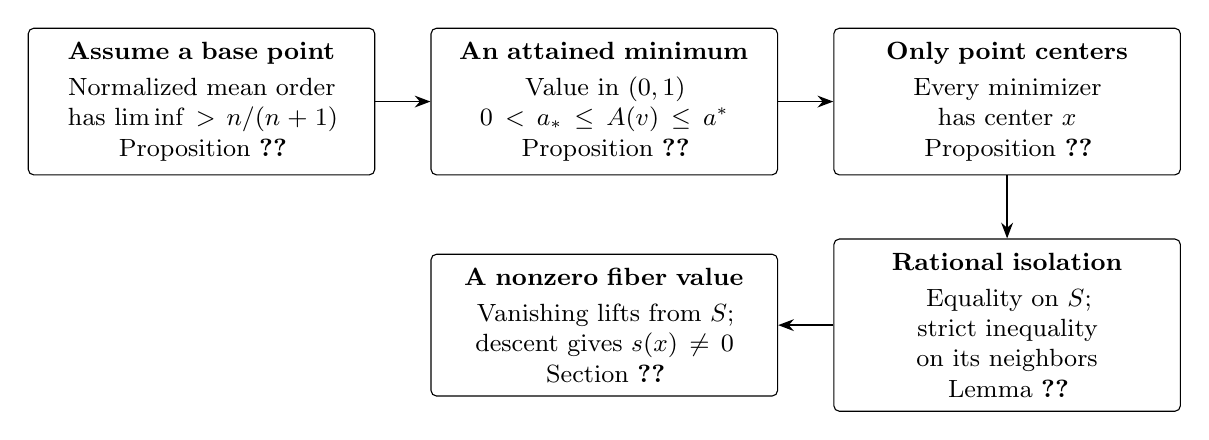
\begin{tikzpicture}[
  box/.style={draw,rounded corners=2pt,align=center,text width=4.05cm,
    minimum height=1.65cm,inner sep=5pt,font=\small},
  flow/.style={-{Stealth[length=2mm]},semithick}]
\node[box] (gap) {\textbf{Assume a base point}\\[2pt]
  Normalized mean order\\
  has $\liminf>n/(n+1)$\\
  Proposition~\ref{prop:ordinary-gap}};
\node[box,right=7mm of gap] (minimum) {\textbf{An attained minimum}\\[2pt]
  Value in $(0,1)$\\
  $0<a_*\leq\A(v)\leq a^*$\\
  Proposition~\ref{prop:minimizers}};
\node[box,right=7mm of minimum] (point) {\textbf{Only point centers}\\[2pt]
  Every minimizer has center $x$\\
  Proposition~\ref{prop:point-center}};
\node[box,below=8mm of point] (isolation) {\textbf{Rational isolation}\\[2pt]
  Equality on $S$;\\
  strict inequality\\
  on its neighbors\\
  Lemma~\ref{lem:isolated-equality}};
\node[box,left=7mm of isolation] (lift) {\textbf{A nonzero fiber value}\\[2pt]
  Vanishing lifts from $S$; descent gives $s(x)\ne0$\\
  Section~\ref{sec:final-lift}};
\draw[flow] (gap) -- (minimum);
\draw[flow] (minimum) -- (point);
\draw[flow] (point) -- (isolation);
\draw[flow] (isolation) -- (lift);
\end{tikzpicture}
\caption{The contradiction proving the sharp adjoint bound.
The discrepancy bounds are uniform before fixing $t<n+1$; for that one
parameter, every minimizer has point center in arbitrarily large degrees.
Here $S$ is the reduced divisor over $x$ on which the constructed
boundary coefficient equals log discrepancy.}
\label{fig:proof-route}
\end{figure}


\section{Orders, thresholds, and vanishing}\label{sec:preliminaries}
Throughout the proof, $X$, $L$, and $n$ satisfy the hypotheses of
Theorem~\ref{thm:main}. Write
\[
 P=K_X+(n+1)L,\qquad R_j=H^0(X,jL),\qquad N_j=\dim R_j.
\]
Ampleness gives
\begin{equation}\label{eq:hilbert-X}
 N_j=\frac{L^n}{n!}j^n+O(j^{n-1}),\qquad L^n\geq1.
\end{equation}
All centers are \emph{closed} centers. Thus a divisor centered along
a subvariety $W$ is an admissible test at every point of $W$, not just
at its generic point.

\subsection{Weighted orders}
We use resolution and principalization in characteristic zero with a
prescribed simple normal crossing (SNC) boundary; see
\cite[Theorems~1.0.1 and~2.4.1]{wlodarczyk2005}.
Models used for vanishing are projective. We may resolve above an
already chosen model and retain any previously extracted prime by its
strict transform.

For a prime divisor $F$ on a smooth birational model $\pi:Y\to X$,
the log discrepancy is
\[
 \A(F)=1+\ord_F(K_{Y/X}).
\]
We permit positive multiples of $\ord_F$ and scale discrepancy by the
same multiple. Orders of sections mean orders of their effective zero
divisors; orders of ideals mean the minimum of the orders of local
generators. A local frame pulled back from $X$ may be used in these
calculations.

We also use weighted monomial orders. Choose a smooth projective
birational model and local regular coordinates adapted to the
\emph{entire} relative canonical divisor: every component of that
divisor meeting the coordinate neighborhood is a coordinate
hyperplane. All coordinate divisors used below, together with that
support, must form a simple normal crossing divisor. Choose a subset
$E_1,\ldots,E_r$ of the coordinate divisors and give it positive real
weights $u_1,\ldots,u_r$; the remaining coordinates have weight zero.
The order of a germ is the least weight of a nonzero
monomial in their local equations, with coefficients in the remaining
coordinates, and
\begin{equation}\label{eq:monomial-discrepancy}
             \A(v)=\sum_{j=1}^r u_j\A(E_j).
\end{equation}
A coordinate divisor absent from the relative canonical divisor has
log discrepancy one. We use a chosen irreducible component of the
positive-support stratum, whose generic point avoids all zero-weight
coordinate divisors; its closed image is the center on $X$. This
adaptation condition is essential for
\eqref{eq:monomial-discrepancy}. The test with all weights zero is
excluded.

For positive rational weights this is a divisorial order up to scale.
Indeed, clearing denominators and extracting the corresponding
primitive ray is a toroidal modification in regular parameters. The
relative canonical order in those parameters is the sum of the
primitive weights minus one. Adding the pullback of the previous
relative canonical divisor gives
\eqref{eq:monomial-discrepancy}. The extraction can be retained on a
smooth projective model by resolution. Approximating weights on a
fixed support by positive rational weights approximates both
discrepancy and the orders of any fixed finite collection of sections.
For the latter assertion only finitely many coordinatewise minimal
exponents need be considered.

\begin{lemma}[Local computation of a monomial order]\label{lem:monomial-local}
A monomial order with fixed positive support can be computed in the
Taylor ring at any smooth point of its open stratum. Its value is
unchanged by replacing each positive-weight coordinate by a unit
multiple or by changing the complementary zero-weight coordinates.
\end{lemma}
\begin{proof}
For a positive threshold $c$, the corresponding ideal is generated by
the monomials in the positive-weight parameters of weight at least
$c$. These generators are preserved, up to units, under the stated
changes. In the completed local ring the ideal is extended from a
finite-colength monomial ideal in the positive-weight variables. It
is therefore primary to their intersection. Localization at the
generic point of that stratum followed by contraction does not change
membership. The same conclusion in the regular local ring follows
from faithful flatness of completion. In particular a coefficient
which vanishes at the chosen closed point, but not identically on the
stratum, is still a nonzero series in zero-weight variables; it does
not raise the old weighted order.
\end{proof}

\begin{lemma}[SNC retraction]\label{lem:retraction}
Let $D_1,\ldots,D_N$ be effective divisors on $X$, and let $Y\to X$
be a log resolution of their union. Include all exceptional divisors
in its SNC divisor, with components $E_j$. For any positive multiple
$v$ of a prime-divisor order over $Y$, set $u_j=v(E_j)$. Then
\begin{equation}\label{eq:retraction}
 v(D_i)=\sum_j u_j\ord_{E_j}(D_i),\qquad
 \A(v)\geq\sum_j u_j\A(E_j).
\end{equation}
If some $u_j$ is nonzero, the monomial order with these weights at the
stratum containing the generic center of $v$ has the same orders on
the $D_i$, no larger discrepancy, and a closed center on $X$
containing that of $v$.
\end{lemma}
\begin{proof}
Each pulled-back divisor is locally a monomial times a unit, which
gives the first equality. The reduced SNC divisor on $Y$ is log
canonical: equivalently, a logarithmic volume form has at most a
simple pole along every prime on a higher smooth model. Thus the
log discrepancy over $Y$ is at least $\sum_j u_j$. Adding the order of
$K_{Y/X}$ gives the second inequality and the claimed discrepancy
of the monomial order. The stratum closure contains the generic
center, so its proper image contains the original closed center.
\end{proof}

\subsection{Thresholds in families}
For a coherent ideal $\mathfrak a$ on a smooth variety, its local log
canonical threshold at $x$ is computed on a log resolution by
\begin{equation}\label{eq:lct-formula}
 \lct_x(\mathfrak a)=
 \min_{x\in\pi(F),\,\ord_F(\mathfrak a)>0}
       \frac{\A(F)}{\ord_F(\mathfrak a)}.
\end{equation}
The minimum is $+\infty$ for the unit ideal. For the zero ideal the
threshold is zero. The same formula follows by change of variables
from local integrability of
$(\sum |g_i|^2)^{-c}$ for generators $g_i$ of $\mathfrak a$.

\begin{lemma}[Closed threshold loci]\label{lem:lct-family}
Let $V$ be a smooth complex projective variety, let $S$ be a complex
algebraic variety, and let $\mathfrak a$ be an ideal on $V\times S$
locally given by algebraic families of generators. For a real number
$c$, the locus
\[
 \{(x,s):\lct_x(\mathfrak a_s)\leq c\}
\]
is Zariski closed. Here $\mathfrak a_s$ denotes the ideal generated
by the restricted generators, with no flatness requirement on its
zero scheme.
\end{lemma}
\begin{proof}
Locally embed the parameter space in a smooth space and extend the
finitely many generators holomorphically to a coordinate neighborhood
of that ambient space. The analytic semicontinuity of complex
singularity exponents applies to
$\varphi=\tfrac12\log\sum |g_i|^2$ there and hence on $S$;
$e^{\varphi}$ is locally H\"older continuous. In local coordinates,
translation of the variable handles a moving marked point.
Consequently the displayed locus is closed in the classical
topology; see \cite[Lemma~3.2]{dk2001}.

It is also algebraically constructible. The following generic-resolution
stratification argument parallels the proof of
\cite[Theorem~3.1]{dk2001}. Resolve the ideal over the
generic point of each irreducible component of $S$ and spread the
resolution over a dense open subset. After shrinking, generic
smoothness makes the fibers and all relevant crossings smooth, so
the fiber maps are log resolutions with fixed orders and
discrepancy coefficients. Formula~\eqref{eq:lct-formula} expresses
the threshold condition as a finite union of images of the
relevant divisors on this piece. These images are algebraic because
the resolution is proper. A finite cover used to separate
components preserves constructibility of the image. Induction on
the closed complement gives a finite stratification and proves
constructibility on $V\times S$. The zero-ideal case is separated
as an algebraic condition. In dimension zero the assertion follows
directly from the vanishing of the generators.

A constructible subset of a complex algebraic variety which is
classically closed is Zariski closed: every Zariski open subset of
an irreducible closed subvariety is classically dense there. This
proves the assertion.
\end{proof}

\subsection{Vanishing and descent}
The cohomological input is Kawamata--Viehweg vanishing
\cite{kawamata1982,viehweg1982}, in the following rounding formulation
\cite[Theorem~0.1]{fujinoKV}.

\begin{theorem}[Kawamata--Viehweg vanishing]\label{thm:kv}
Let $T$ be smooth and projective over $\C$. Let $\Delta$ be an
effective rational SNC divisor with coefficients in $[0,1)$, and
let $D$ be an integral divisor. If $D-(K_T+\Delta)$ is nef and big,
then $H^i(T,\cO_T(D))=0$ for every $i>0$.
\end{theorem}

This is the rounding formulation with
$Q=D-K_T-\Delta$: its fractional support is SNC and
$K_T+\ceil{Q}=D$. In particular, for an integral divisor $M$ and an
effective rational SNC divisor $B$, nefness and bigness of $M-B$
give vanishing for $K_T+M-\floor{B}$, by taking $\Delta=\{B\}$.

We will repeatedly use the following elementary descent observation.
\begin{lemma}\label{lem:descent}
Let $\pi:T\to V$ be a proper birational morphism of smooth varieties,
let $P_V$ be a line bundle on $V$, and let $C$ be an integral divisor
on $T$ whose positive part is exceptional. A section of
$\pi^*P_V+C$ defines a regular section of $P_V$ on $V$.
If a prime $F$ on $T$ maps to a point $x$, the coefficient of $C$
on $F$ is zero, and the section is nonzero generically on $F$, then
the descended section is nonzero at $x$.
\end{lemma}
\begin{proof}
View the section as a rational section of $P_V$ on the common
function field. Its orders on all nonexceptional primes are
nonnegative, since the coefficients of $C$ there are nonpositive.
It is therefore regular in codimension one on the normal variety
$V$, and hence everywhere. Under the additional assumptions its
pullback has order zero along $F$. A local function vanishing at
$x$ has positive order along every prime centered at $x$, so the
descended section cannot vanish at $x$.
\end{proof}

\section{The ordinary-order alternative}
\label{sec:min-ordinary}

This section converts failure of adjoint generation at a point into a
strict asymptotic inequality for ordinary orders. Lattice counting gives
the non-strict bound; the main task is to show that its equality case
already permits a nonzero fiber value to be lifted.

Fix a closed point $x\in X$. Choose regular parameters at $x$ and a
local frame of $L$, using its powers as frames of $jL$. We order Taylor
monomials first by total degree and then lexicographically, always taking
the smallest monomial. Let
\[
 H_j=\{\operatorname{in}(s):0\ne s\in R_j\}
       \subset\Z_{\geq0}^n
\]
be the set of initial exponents. Thus
$|\operatorname{in}(s)|_1=\mult_x(s)$.

The equality between the number of initial exponents and the dimension
of the section space is the elementary counting principle in
\cite[Lemma~1.4]{lazarsfeldmustata2009} and
\cite[Proposition~2.6]{kavehkhovanskii2012}.
We include its proof for the order chosen here.

\begin{lemma}
\label{lem:min-initials}
The set $H_j$ has cardinality $N_j$, and representatives of its distinct
exponents form a basis of $R_j$. There is a constant $C>0$, independent
of $j$ and $s$, such that
\begin{equation}
\label{eq:min-multiplicity}
 \mult_x(s)\leq Cj\qquad(0\ne s\in R_j).
\end{equation}
Moreover $H_j+H_q\subset H_{j+q}$.
\end{lemma}

\begin{proof}
Taylor expansion is injective on $R_j$: a section with zero germ vanishes
on a nonempty open set and hence on the integral variety $X$. Each
monomial coefficient has a one-dimensional space of possible values.
Successively selecting a smallest initial monomial and eliminating its
coefficient from the remaining basis vectors therefore produces a basis
with distinct initials. Any linear combination of these vectors has the
initial of its first nonzero summand in this ordering. This proves the
cardinality assertion.

Choose a fixed sufficiently ample multiple $kL$. General members of its
linear system through $x$ cut out a curve smooth at $x$ and not contained
in the divisor of a prescribed nonzero section of $jL$. Local
intersection multiplicity bounds $\mult_x(s)$ from above by the degree
of that divisor on the curve, at most $jk^{n-1}L^n$. The same assertion
in dimension one is simply the degree bound for an effective divisor
on $X$. This gives \eqref{eq:min-multiplicity}. Finally, the chosen
monomial ordering is multiplicative, so initial exponents add under
products of sections.
\end{proof}

\begin{proposition}[Ordinary-order alternative]
\label{prop:ordinary-gap}
If $P$ is not generated by its global sections at $x$, then
\begin{equation}
\label{eq:min-gap}
 \liminf_{j\longrightarrow\infty}
   \frac{1}{jN_j}\sum_{\gamma\in H_j}|\gamma|_1
       >\frac{n}{n+1}.
\end{equation}
\end{proposition}

\begin{proof}
We prove that failure of the strict inequality implies generation at
$x$. The proof has three steps: lattice equality forces volume one,
the resulting leading forms give a strict threshold on the exceptional
divisor of the point blowup, and vanishing lifts a nonzero section from
that divisor. Put $V=L^n$. The number of nonnegative integral points of total
degree at most $r$ is $\binom{r+n}{n}$. Filling the points in order of
increasing total degree, and using
$N_j=Vj^n/n!+O(j^{n-1})$, gives
\begin{equation}
\label{eq:min-lattice-lower}
 \liminf_{j\longrightarrow\infty}
 \frac{1}{jN_j}\sum_{\gamma\in H_j}|\gamma|_1
 \geq V^{1/n}\frac{n}{n+1}.
\end{equation}
Indeed the last occupied degree for a set of $N_j$ smallest points is
$V^{1/n}j+O(1)$, and summing total degree over these points gives mean
degree $V^{1/n}nj/(n+1)+O(1)$. Since $V$ is a positive integer, failure
of \eqref{eq:min-gap} forces $V=1$ and equality along a subsequence.

Let
\[
 \Delta=\{u\in\R_{\geq0}^n:|u|_1\leq1\}.
\]
Along this subsequence, every fixed open ball with closure in the
interior of $\Delta$ meets $j^{-1}H_j$ for all sufficiently large $j$.
To see this, compare $H_j$ with a set $T_j$ of $N_j$ smallest lattice
points. If such a ball were missed, at least $c_1j^n$ points of $T_j$
of degrees at most $(1-c_2)j$ would be absent, for fixed positive
$c_1,c_2$. Every replacement outside $T_j$ has degree at least
$j-O(1)$. The remaining replacements cannot decrease the degree sum,
by the definition of $T_j$. The normalized mean would therefore exceed
the minimum by a fixed positive amount, contradicting equality along
the subsequence.

Choose a rational number $t'$ with $n<t'<n+1$ and put
$c=(1/t',\ldots,1/t')$. This point is in the interior of $\Delta$.
Choose finitely many small balls whose closures lie there and such that
any choice of one point from each ball has convex hull containing $c$
in its interior. For one sufficiently large degree $j$ on the
subsequence, choose initial exponents $\gamma_\nu\in H_j$ in these
balls after scaling by $j^{-1}$. The rational polytope
\[
 Q=\conv\{\gamma_\nu/j\}
\]
contains $c$ in its interior. Its intersection with
$\{|u|_1=n/t'\}$ has rational points $p_1,\ldots,p_b$ whose convex
hull contains $c$ in its interior relative to this full slice
hyperplane. In dimension one this slice is the singleton $\{c\}$.

Write each $p_\ell$ as a rational convex combination of the
$\gamma_\nu/j$, and choose sections $s_\nu$ with those initials.
If $t'=a/b'$ in lowest terms, choose a positive integer $Q_0$ divisible
by $a$ and by every denominator in these convex combinations. Taking
the corresponding products of $Q_0$ sections gives sections
$r_1,\ldots,r_b$ of $jQ_0L$. Set $h=jQ_0/t'$, which is a positive
integer by construction. Their initial exponents $\beta_\ell$ satisfy
\begin{equation}
\label{eq:min-product-initials}
 r_\ell\in H^0(X,ht'L),\qquad
 \beta_\ell=jQ_0p_\ell,\qquad |\beta_\ell|_1=nh.
\end{equation}
In particular, $\conv\{\beta_\ell/h\}$ contains
$\mathbf1=(1,\ldots,1)$ in relative interior in the full hyperplane
$\{|u|_1=n\}$.

Let $p:B=\Bl_xX\longrightarrow X$ and
$E\simeq\mathbb P^{n-1}$ be the exceptional divisor. When $n=1$, take
$p$ to be the identity and $E=x$. Removing the common order $nh$ from
the pullbacks of the $r_\ell$ gives a subsystem of
\[
 H=p^*(ht'L)-nhE
\]
with base ideal $\mathfrak b$. Its restriction to $E$ is generated,
in local frames, by the leading homogeneous forms $g_\ell$ of the
$r_\ell$, each of degree $nh$. We claim that
\begin{equation}
\label{eq:min-restricted-threshold}
 \lct_z(E,\mathfrak b|_E)>1/h\qquad(z\in E).
\end{equation}
Here the restricted ideal means its image in $\cO_E$. For $n=1$ it
is the unit ideal, so the assertion holds immediately.

The monomial threshold step below is the unit-monomial special case
of Howald's multiplier-ideal formula~\cite[Main Theorem]{howald2001};
we give the direct SNC argument in this setting.

For $n>1$, first replace the $g_\ell$ by their initial monomials
$z^{\beta_\ell}$. On the affine chart of $E$ where $z_k\ne0$, their
exponents are obtained by omitting coordinate $k$. Projection from
the hyperplane $|u|_1=n$ is an affine isomorphism, so the resulting
normalized exponent polytope contains the all-ones vector in ordinary
interior. Consequently, for every nonzero
$u\in\R_{\geq0}^{n-1}$,
\begin{equation}
\label{eq:min-monomial-strict}
 \frac1h\min_\ell\langle u,\beta_\ell^{(k)}\rangle
       <\sum_i u_i.
\end{equation}
For a prime-divisor order over this chart, use its values on the
coordinate functions as $u$. The left side is the order of the
monomial ideal divided by $h$, while the right side is at most the log
discrepancy, by the SNC inequality in Lemma~\ref{lem:retraction}. If
$u=0$, the ideal order is zero and the discrepancy is positive. Thus
the monomial ideal is klt at coefficient $1/h$. Computing its threshold
on a log resolution, where a finite minimum suffices, gives a strict
threshold greater than $1/h$ at every point.

This statement transfers to the original forms by an algebraic
degeneration. Since only finitely many monomials occur, choose an
integral weight vector $w$ which makes the lexicographic initial of
each $g_\ell$ its unique term of smallest weight. The forms
\[
 g_{\ell,\lambda}(z)
   =\lambda^{-\langle w,\beta_\ell\rangle}
      g_\ell(\lambda^{w_1}z_1,\ldots,\lambda^{w_n}z_n)
\]
have polynomial coefficients in $\lambda$, with monomial special
fiber. They define an algebraic family of ideals on
$E\times\mathbb A^1$. By Lemma~\ref{lem:lct-family}, the locus where
the fiber threshold is at most $1/h$ is closed. Its image in
$\mathbb A^1$ is closed because $E$ is proper, and does not contain
$0$. For some nonzero parameter the threshold is therefore greater
than $1/h$ everywhere on $E$. All nonzero fibers are obtained from the
original forms by a diagonal automorphism of $E$ and nonzero scalar
changes of generators. This proves
\eqref{eq:min-restricted-threshold}. This application uses precisely
the family semicontinuity of complex singularity exponents
\cite{dk2001} incorporated in Lemma~\ref{lem:lct-family}.

It remains to lift from $E$. The blowup formula gives
\begin{equation}
\label{eq:min-adjoint-identity}
 p^*P-(K_B+E)-H/h=(n+1-t')p^*L.
\end{equation}
Take a projective log resolution
$\sigma:T\longrightarrow B$ of $E$ and $\mathfrak b$, with strict
transform $E'$ and
$\mathfrak b\cO_T=\cO_T(-G)$. The divisor $E'$ is not a component
of $G$, since the restricted system is not identically zero. Set
\[
 D_T=K_T+\sigma^*(p^*P-K_B-E)-\lfloor G/h\rfloor.
\]
This is an integral divisor, and
\begin{equation}
\label{eq:min-preliminary-positivity}
 D_T-K_T-\{G/h\}
 =(n+1-t')(p\sigma)^*L+(\sigma^*H-G)/h.
\end{equation}
The first summand is nef and big and the second is nef, because
$\sigma^*H-G$ is globally generated. The fractional boundary has SNC
support. Theorem~\ref{thm:kv}, in the stated logarithmic form of
Kawamata--Viehweg vanishing \cite{fujinoKV}, therefore gives
$H^1(T,\cO_T(D_T))=0$.

Let $\sigma_E:E'\longrightarrow E$ be the induced morphism. Adjunction
identifies the restriction of $D_T+E'$ with
\begin{equation}
\label{eq:min-preliminary-restriction}
 \sigma_E^*(p^*P|_E)
   +K_{E'/E}-\lfloor G|_{E'}/h\rfloor.
\end{equation}
Indeed $E'+\Supp(G)$ is SNC. Each component restricts with
multiplicity one, and two distinct components cannot restrict to the
same prime divisor on $E'$, so taking floors commutes with restriction.
The generators on $E'$ generate $\cO_{E'}(-G|_{E'})$, the pullback
of the restricted ideal. The strict threshold in
\eqref{eq:min-restricted-threshold} implies
\[
 K_{E'/E}-\lfloor G|_{E'}/h\rfloor\geq0.
\]
The first line bundle in \eqref{eq:min-preliminary-restriction} is
trivial with fiber $P_x$. A nonzero vector in this fiber, multiplied
by the canonical section of the effective correction, gives a section
on $E'$ nonzero at its generic point. The exact sequence for $E'$ and
the vanishing just proved lift it to a section of $D_T+E'$.

Relative to $\sigma^*p^*P$, the correction of this lifted bundle is
\[
 C_T=K_{T/B}-\sigma^*E+E'-\lfloor G/h\rfloor.
\]
Its coefficient on $E'$ is zero, and its coefficients on every other
$\sigma$-nonexceptional divisor are nonpositive. Its positive part is
therefore exceptional over $X$. Since $E'$ maps to $x$ and the lifted
section is nonzero at its generic point, Lemma~\ref{lem:descent}, applied
to $p\sigma$, gives a section of $P$ nonzero at $x$. This proves the
proposition, including dimension one, when $E'$ is the point itself.
\end{proof}

\section{Finite-degree exponential minimization}
\label{sec:min-exponential}

We now allow both the basis and the monomial test to vary. The strict
ordinary-order inequality makes the objective less than one, and a
supply of low-order jets bounds the discrepancy on that sublevel set.
To prove attainment, we first select one flag and its adapted basis;
only then do we choose the resolution on which compactness is used.

For $N_m>0$, an ordered basis $\mathbf s=(s_1,\ldots,s_{N_m})$ of
$R_m$, a nonzero monomial test $v$, and $t>0$, put
\begin{equation}
\label{eq:min-objective}
 F_{m,t}(v,\mathbf s)
  =\frac1{N_m}\sum_{i=1}^{N_m}
       \exp\!\left(\frac{\A(v)}t-\frac{v(s_i)}m\right),
 \qquad
 f_{m,t}(z)=\inf_{\substack{v,\mathbf s\\z\in c_X(v)}}
                F_{m,t}(v,\mathbf s).
\end{equation}
Here $c_X(v)$ denotes the closed center, and the infimum also ranges
over the bases. Positive rescaling of a test is always allowed.
Approximating its positive weights by rational weights preserves its
center and approximates the orders of finitely many sections and its
discrepancy. Thus the same infimum is obtained using positive multiples
of prime-divisor orders.

\begin{lemma}
\label{lem:min-order-bound}
If the center of a test $v$ contains $x$, then every nonzero section
$s$ satisfies
\begin{equation}
\label{eq:min-order-bound}
 v(s)\leq\A(v)\mult_x(s).
\end{equation}
In particular, for $s\in R_m$ one has
$0\leq v(s)/\A(v)\leq Cm$, with $C$ as in
Lemma~\ref{lem:min-initials}.
\end{lemma}

\begin{proof}
For an effective divisor with local equation $g$ of multiplicity $r>0$
at a smooth point, the elementary bound
$\lct_x(g)\geq1/r$ suffices. One analytic proof uses Weierstrass
preparation in a general coordinate direction. On a smaller
polydisc, $g$ is a unit times a monic polynomial of degree $r$ in that
coordinate. For any $c<1/r$, factor this polynomial into its $r$
complex roots for each fixed choice of the other coordinates. H\"older's
inequality bounds the integral of its absolute value to the power
$-2c$ by the product of integrals with exponents $-2cr$. These
one-variable integrals are uniformly finite because $cr<1$ and the
roots remain bounded. Fubini's theorem proves local integrability.
The unit case has infinite threshold. Computing the threshold on a
log resolution now gives \eqref{eq:min-order-bound} for divisorial
orders with centers containing $x$, and rational approximation gives
it for the admitted monomial tests.
\end{proof}

\begin{lemma}[Uniform sublevel bounds]
\label{lem:min-coercivity}
Suppose that $P$ is not generated at $x$. There are numbers
$0<t_0<n+1$, $c>0$, $0<\delta<1$, $0<a_*\leq a^*<\infty$, and
an integer $m_0$ such that, for every $m\geq m_0$ and every
$t\in[t_0,n+1]$,
\begin{equation}
\label{eq:min-uniform-bounds}
 c\leq f_{m,t}(x)\leq1-\delta.
\end{equation}
Moreover, any pair in \eqref{eq:min-objective} centered with image
containing $x$ and satisfying
$F_{m,t}(v,\mathbf s)\leq1-\delta/2$ has
\begin{equation}
\label{eq:min-discrepancy-bounds}
 a_*\leq\A(v)\leq a^*.
\end{equation}
All these constants are independent of $m$ and $t$ in the indicated
ranges.
\end{lemma}

\begin{proof}
By Proposition~\ref{prop:ordinary-gap}, there is $\epsilon>0$ such
that, for all sufficiently large $m$,
\[
 \frac1{mN_m}\sum_{\gamma\in H_m}|\gamma|_1
       \geq\frac n{n+1}+3\epsilon.
\]
Choose $t_0<n+1$ sufficiently close that
$n/t_0\leq n/(n+1)+\epsilon$. Take a basis with distinct ordinary
initials, and use $v=\lambda\ord_x$, where $\ord_x$ is the
ordinary point order and $\A(\ord_x)=n$. In dimension one this is
the order of the point itself. The linear coefficient at $\lambda=0$
in its objective is at most $-2\epsilon$, uniformly in $m$ and $t$.
By \eqref{eq:min-multiplicity}, the quantities
$n/t-\mult_x(s_i)/m$ are uniformly bounded, so the quadratic remainder
in their exponential expansion is uniformly $O(\lambda^2)$. A fixed
sufficiently small $\lambda>0$ therefore gives
$F_{m,t}\leq1-\delta$ for a fixed $\delta>0$.

We next give a uniform supply of low-order jets. Choose $k>0$ such that
$kL$ is very ample, and sections $s_0,s_1,\ldots,s_n$ of $kL$ such
that $s_0(x)\ne0$ and $z_i=s_i/s_0$ are regular parameters at $x$.
For each residue class modulo $k$, choose a fixed sufficiently large
integer $b_r$ in that class for which $b_rL$ is globally generated,
and choose $\tau_r\in H^0(X,b_rL)$ nonzero at $x$. Write
$m=qk+b_r$ using the corresponding residue. For $|\alpha|_1\leq q$,
the sections
\[
 \tau_r s_0^{q-|\alpha|_1}s_1^{\alpha_1}\cdots s_n^{\alpha_n}
\]
have germs equal to a common unit times $z^\alpha$ in a local frame
of $mL$. In particular, if
\[
 r_m=\min\left(q,\left\lfloor\frac{m}{2(n+1)}\right\rfloor\right),
\]
their jets for $|\alpha|_1\leq r_m$ are linearly independent modulo
ordinary order greater than $m/(2t)$. For large $m$, $r_m$ is at least
a fixed positive multiple of $m$. The Hilbert asymptotic consequently
gives a constant $0<\kappa<1$, independent of $m,t$, with
\begin{equation}
\label{eq:min-jet-codimension}
 \codim_{R_m}\{s:\mult_x(s)>m/(2t)\}\geq\kappa N_m.
\end{equation}

Put $a=\A(v)$. By Lemma~\ref{lem:min-order-bound}, the subspace
$\{s:v(s)>ma/(2t)\}$ is contained in the subspace in
\eqref{eq:min-jet-codimension}. Thus at least $\kappa N_m$ vectors
of any basis, whether or not it is adapted to $v$, have
$v(s_i)\leq ma/(2t)$. It follows that
\begin{equation}
\label{eq:min-coercive-exponential}
 F_{m,t}(v,\mathbf s)
   \geq\kappa\exp\!\left(\frac a{2t}\right)
   \geq\kappa\exp\!\left(\frac a{2(n+1)}\right).
\end{equation}
This proves the lower bound in \eqref{eq:min-uniform-bounds}, with
$c=\kappa$, and bounds $a$ above on the stated sublevel set.

Finally, \eqref{eq:min-order-bound} and
\eqref{eq:min-multiplicity} show that
$F_{m,t}(v,\mathbf s)\geq e^{-Ca}$. Choose $a_*>0$ sufficiently
small that $e^{-Ca_*}>1-\delta/2$. No pair in the sublevel set can
have $a<a_*$. Enlarging the upper bound if necessary gives
$a^*\geq a_*$ and proves all the assertions.
\end{proof}

\begin{lemma}[Closed realizability loci]
\label{lem:min-flags}
Fix $m$ with $N_m>0$ and a decreasing list
$\alpha_1\geq\cdots\geq\alpha_{N_m}\geq0$ of rational numbers.
The set of points $z\in X$ for which some ordered basis and some
prime-divisor order $v$, with $z\in c_X(v)$, satisfy
\begin{equation}
\label{eq:min-rational-list}
 \frac{v(s_i)}{\A(v)}\geq\alpha_i
       \qquad(1\leq i\leq N_m)
\end{equation}
is Zariski closed. There is also a closed incidence locus in the
product of $X$ with the complete flag variety of $R_m$ recording
realizability by bases adapted to a given flag.
\end{lemma}

\begin{proof}
Let $\mathcal F$ be that projective flag variety. A flag has subspaces
$U_i\subset R_m$ of dimensions $i$ and associated base ideals
$\mathfrak b_i\subset\cO_X$, obtained by evaluation after twisting
by $-mL$. If \eqref{eq:min-rational-list} holds, the flag spanned by
the first $i$ basis vectors satisfies
\begin{equation}
\label{eq:min-flag-inequalities}
 v(\mathfrak b_i)\geq\alpha_i\A(v)
       \qquad(1\leq i\leq N_m),
\end{equation}
since the list is decreasing. Conversely these inequalities imply
\eqref{eq:min-rational-list} for every basis adapted to the flag.

If at least one $\alpha_i$ is positive, choose a positive integer $M$
such that $M/\alpha_i$ is integral for every positive entry, and set
\[
 \mathfrak a_\alpha
    =\sum_{i:\alpha_i>0}\mathfrak b_i^{\,M/\alpha_i}.
\]
The simultaneous inequalities \eqref{eq:min-flag-inequalities} are
equivalent to $v(\mathfrak a_\alpha)\geq M\A(v)$. A divisorial
witness with center containing $z$ exists if and only if
\begin{equation}
\label{eq:min-flag-threshold}
 \lct_z(X,\mathfrak a_\alpha)\leq1/M,
\end{equation}
because the local threshold is computed by a component on a log
resolution. The universal subbundles on $\mathcal F$ give algebraic
families of generators for the base ideals on $X\times\mathcal F$,
and hence for their indicated powers and sum. Lemma~\ref{lem:lct-family}
applied to \eqref{eq:min-flag-threshold} gives the closed incidence
locus. Its projection to $X$ is closed by properness of $\mathcal F$.
If all entries vanish, both loci are the whole parameter spaces.
\end{proof}

\begin{proposition}[Existence and uniform bounds for minimizers]
\label{prop:minimizers}
Suppose that $P$ is not generated at $x$. For the constants and ranges
in Lemma~\ref{lem:min-coercivity}, $f_{m,t}(x)$ satisfies
\eqref{eq:min-uniform-bounds} and is attained by an ordered basis
of $R_m$ and a nonzero real-weight monomial test on a projective log
resolution of the divisors of that basis. Every minimizing test has
\[
 a_*\leq\A(v)\leq a^*.
\]
More generally the same bounds hold eventually along every minimizing
sequence. In particular, the positive lower bound $a_*$ is independent
of $m\geq m_0$ and $t\in[t_0,n+1]$.
\end{proposition}

\begin{proof}
Only attainment remains to be proved. Fix $m,t$ in the indicated
ranges and take a sequence of divisorial pairs whose objectives
decrease to $f_{m,t}(x)$. Eventually they lie in the sublevel set of
Lemma~\ref{lem:min-coercivity}. Order each basis by decreasing
normalized values and pass to a subsequence for which
\[
 a_b=\A(v_b)\longrightarrow a\in[a_*,a^*],\qquad
 q_{b,i}=\frac{v_b(s_{b,i})}{\A(v_b)}\longrightarrow q_i.
\]
This is possible because $0\leq q_{b,i}\leq Cm$. The limit list is
decreasing and
\begin{equation}
\label{eq:min-limit-objective}
 f_{m,t}(x)=\frac1{N_m}\sum_i
       \exp\!\left(\frac at-\frac{aq_i}m\right).
\end{equation}
At least one $q_i$ is positive: otherwise the right side would be
$e^{a/t}>1$, contrary to \eqref{eq:min-uniform-bounds}.

Choose decreasing nonnegative rational lists
$\alpha^{(k)}=(\alpha_i^{(k)})$ which increase componentwise to
$(q_i)$ and are strictly below $q_i$ whenever $q_i>0$. Each list is
satisfied by all sufficiently late pairs in the minimizing sequence.
By the incidence assertion of Lemma~\ref{lem:min-flags}, the flags
admitting a divisorial witness at $x$ for that list form a nonempty
closed subset $\mathcal F_k$ of $\mathcal F$. The subsets are nested,
so projectivity gives a flag in their intersection. Fix a basis
$s_1,\ldots,s_{N_m}$ adapted to this one flag.

Resolve the divisors of these sections on a single smooth projective
model $Y\longrightarrow X$, including the exceptional divisors in
the SNC support. For each sufficiently large $k$, choose a divisorial
witness for the fixed flag and the list $\alpha^{(k)}$, and exhibit it
on a common smooth model dominating $Y$. Its retraction
to this fixed SNC model, as in Lemma~\ref{lem:retraction}, preserves
all the section orders, cannot increase discrepancy, and has center
on $X$ containing $x$. The retraction is nonzero because the list
has a positive entry. Normalize it to discrepancy one. It then
satisfies
\begin{equation}
\label{eq:min-retracted-lists}
 \widetilde v_k(s_i)\geq\alpha_i^{(k)}
       \qquad(1\leq i\leq N_m).
\end{equation}

There are finitely many SNC strata and their components on $Y$.
After passing to a subsequence, the retractions use the same stratum
component, with coordinate divisors indexed by a fixed set $J$.
Their normalized weights belong to the compact simplex
\[
 \left\{(u_j)_{j\in J}:u_j\geq0,\quad
                \sum_{j\in J}\A(E_j)u_j=1\right\};
\]
all coefficients $\A(E_j)$ are strictly positive because $X$ is
smooth. Pass to a limit of the weights. A weight may become zero.
We take the component of the remaining positive-support intersection
that contains the old stratum component. Its closure contains the old
center, so its image still contains $x$.
The limit is a nonzero monomial test $\widetilde v$
of discrepancy one. On the fixed resolution, the section orders are
linear in these weights. Consequently
\eqref{eq:min-retracted-lists} gives
$\widetilde v(s_i)\geq q_i$ for every $i$.

Set $v=a\widetilde v$. Comparing with
\eqref{eq:min-limit-objective} yields
\[
 F_{m,t}(v,\mathbf s)
 \leq\frac1{N_m}\sum_i
       \exp\!\left(\frac at-\frac{aq_i}m\right)
 =f_{m,t}(x).
\]
The reverse inequality holds by definition of the infimum, so this
pair attains it. The claimed discrepancy bounds for all minimizers
and eventually for minimizing sequences follow directly from the
uniform sublevel bounds.
\end{proof}

The same closed realizability loci also compare the infimum along a
possible center. This comparison will allow the tangential variation in
Section~\ref{sec:centers} to be tested at a very general point.

\begin{lemma}[Specialization comparison]
\label{lem:specialization}
For fixed $m$ with $N_m>0$, let $W\subset X$ be a closed irreducible
subvariety containing $x$. At a very general closed point $y\in W$,
one has, for every $t>0$,
\begin{equation}
\label{eq:min-specialization}
 f_{m,t}(y)\geq f_{m,t}(x).
\end{equation}
\end{lemma}

\begin{proof}
There are countably many rational lists of the kind in
Lemma~\ref{lem:min-flags}. For each, intersect its closed realizability
locus with $W$, and exclude that intersection if it is proper in $W$.
The complement contains very general closed points over $\C$.
For any remaining $y$, every such list realized at $y$ is realized
at $x$.

Take a divisorial test and a basis at $y$, reorder the basis so that
$q_i=v(s_i)/\A(v)$ is decreasing, and put $a=\A(v)>0$. Approximate
$(q_i)$ componentwise from below by decreasing rational lists
$(\alpha_i^{(b)})$. For each list, choose a realizing pair at $x$ and
scale its test to discrepancy exactly $a$. Its objective is at most
\[
 \frac1{N_m}\sum_i
       \exp\!\left(\frac at-\frac{a\alpha_i^{(b)}}m\right).
\]
Taking the limit gives $f_{m,t}(x)\leq F_{m,t}(v,\mathbf s)$.
Infimizing over the divisorial pairs at $y$ proves
\eqref{eq:min-specialization}. The excluded loci do not depend on
$t$, which explains the simultaneous statement for all positive $t$.
\end{proof}

\section{Eliminating positive-dimensional centers}
\label{sec:centers}

The specialization comparison can be combined with a tangential
variation of a minimizing test. The essential point is that the estimates
for sections on its center are uniform as that center varies.

\begin{proposition}\label{prop:point-center}
Suppose that $P$ is not generated at $x$. There is a real number
$0<t<n+1$ such that, for arbitrarily large integers $m$, the infimum
$f_{m,t}(x)$ is attained and every minimizing monomial pair has center
exactly $\{x\}$.
\end{proposition}

Here a minimizing pair consists of a monomial test and a basis attaining
the infimum. The assertion concerns all such pairs, even if their models,
coordinates, and bases differ. This universal assertion will be needed
in Section~\ref{sec:isolation}: a second test with the same normalized
section orders and discrepancy is also minimizing, so it too must have
point center. We first establish a uniform estimate that will apply to
all possible centers.



\subsection{A uniform estimate on restriction spaces}

Fix a positive integer $k$ such that $kL$ is very ample, and use its
complete system to embed $X$ in a projective space. For an integral
$d$-dimensional closed subvariety $W\subset X$, put
\[
 I_W(h)=\dim_{\C}\im\bigl(R_h\longrightarrow H^0(W,hL|_W)\bigr).
\]
We require a lower estimate for this image, rather than surjectivity of
the restriction map.

\begin{lemma}\label{lem:uniform-restrictions}
For each $1\le d\le n$, there are constants $C_d$ and $H_d$, depending
only on $(X,L,k,d)$, such that
\begin{equation}\label{eq:uniform-restrictions}
 \bigl(d!I_W(h)\bigr)^{1/d}\ge h-C_d
 \qquad(h\ge H_d)
\end{equation}
for every integral $d$-dimensional closed subvariety $W\subset X$.
\end{lemma}

\begin{proof}
Set $D_0=k^d$. The degree of $W$ in the fixed embedding is
\[
 D=(kL)^d\cdot W=k^d(L^d\cdot W)\ge D_0,
\]
because the last intersection number is a positive integer. A general
linear projection gives a finite morphism
$\pi:W\longrightarrow\mathbb P^d$ of degree $D$. Its generic fiber is
separable, since the ground field has characteristic zero. Write
$K=\C(\mathbb P^d)$ and $E=\C(W)$.

Choose a nonzero linear coordinate $s_0$ of the projection. All points of
the geometric generic fiber lie in $s_0\ne0$. Select $D_0$ of these
distinct points. Over an algebraic closure of $K$, affine linear forms
separate any two of them. For each selected point, multiplying at most
$D_0-1$ such forms gives a polynomial vanishing at the other selected
points and not at that one. Homogenizing with $s_0$ gives ambient forms
of degree $D_0$ whose normalized values span the functions on these
$D_0$ points.

Let $V_{D_0}$ be the complex vector space of ambient degree-$D_0$
forms. Restriction and division by $s_0^{D_0}$ define a $K$-linear map
$V_{D_0}\otimes_{\C}K\longrightarrow E$. It has rank at least $D_0$.
Indeed this rank can be checked after extending scalars to the algebraic
closure of $K$, where the preceding evaluation argument applies. We may
therefore choose ambient degree-$D_0$ forms $F_1,\ldots,F_{D_0}$ for which
\[
 F_1/s_0^{D_0},\ldots,F_{D_0}/s_0^{D_0}\in E
\]
are linearly independent over $K$. The forms can be chosen among a fixed
monomial spanning set; their coefficients need not depend on elements
of $K$.

For $q\ge D_0$, multiply each $F_i$ by a monomial basis of the
homogeneous forms of degree $q-D_0$ in the coordinates of the
projection. These products restrict
to linearly independent sections on $W$. In fact, a relation between
them, divided by $s_0^q$, is a relation between the displayed
$K$-independent elements; all its coefficients must vanish in $K$.
The corresponding base forms must then vanish identically on
$\mathbb P^d$. The products are restrictions of sections in $R_{qk}$,
so
\begin{equation}\label{eq:restriction-binomial}
 I_W(qk)\ge D_0\binom{q-D_0+d}{d}.
\end{equation}
In particular,
\begin{equation}\label{eq:restriction-multiples}
 \bigl(d!I_W(qk)\bigr)^{1/d}
 \ge k(q-D_0)=qk-k^{d+1}.
\end{equation}

To cover all degrees, choose, once and for all, an integer $h_r$ in each
residue class $r$ modulo $k$ such that $h_rL$ is globally generated.
There is a section of $h_rL$ not identically zero on any given $W$.
Multiplication by that section injects the degree-$qk$ restriction space
into the degree-$(qk+h_r)$ restriction space, because $W$ is integral.
For $h=qk+h_r$ and $q\ge D_0$, Equation
\eqref{eq:restriction-multiples} thus gives
\[
 \bigl(d!I_W(h)\bigr)^{1/d}
 \ge h-(h_r+k^{d+1}).
\]
Taking maxima over the finitely many residue classes proves the lemma.
For example, both $C_d$ and $H_d$ may be taken to equal
$\max_r h_r+k^{d+1}$. All thresholds and constants are independent
of $W$.
\end{proof}

\subsection{A minimizing test and its tangent directions}

Assume from now on that $P$ is not generated at $x$.
Fix $t\in[t_0,n+1]$ and a sufficiently large degree $m$ in the ranges
of Proposition~\ref{prop:minimizers}, and write $f_j=f_{j,t}(x)$.
Suppose that a minimizing monomial pair has test $v$ and center $W$
of dimension $d>0$. We derive upper and lower bounds for its weighted
tangential moment, keeping $m$ and $t$ fixed in this calculation.
Let $Z$ be the closure of its defining stratum on
a smooth model $Y\to X$, and let $r$ be the number of its positive
weights. Put $k'=n-d$, so $r\le k'$. For the local estimates below,
keep this test, its model, and the coordinates chosen below fixed; section spaces in
every degree $j$ use the same Taylor order.

Choose a very general smooth point $y\in W$ satisfying
Lemma~\ref{lem:specialization} in degree $m$:
\begin{equation}\label{eq:center-specialization}
 f_{m,t}(y)\ge f_{m,t}(x).
\end{equation}
The very general condition and the smooth open sets used below can be
met simultaneously over $\C$. Above $y$ choose a
point $z$ of the open stratum of $Z$ where $Z\to W$ is smooth, avoiding
all additional components of the relative canonical divisor. Generic
smoothness allows these choices. Take regular parameters at $z$ in
three groups:
\begin{enumerate}
 \item the $r$ parameters defining the positive-weight crossing
 components;
 \item $k'-r$ parameters along the fiber of $Z\to W$;
 \item $d$ parameters pulled back from affine linear projective
 coordinates on $W$ vanishing at $y$.
\end{enumerate}
For the last group, choose $d$ independent differentials from the fixed
$kL$ embedding. Complete them by the fiber parameters using the
smoothness of $Z\to W$.

The point $z$ lies in the open positive-support stratum, the positive
equations change only by units, and the complementary parameters have
weight zero. By Lemma~\ref{lem:monomial-local}, the original weighted
order is therefore unchanged and can be computed from Taylor series
at $z$.

Choose a local frame of $L$ near $y$ and pull it back to $Y$. The terms
of a section with all first $r$ exponents zero are its restriction to
$Z$. Since that restriction comes from $W$, its Taylor expansion
depends only on the last $d$ parameters.

Write Taylor exponents as
\[
 (p,\beta)\in\mathbb Z_{\ge0}^{k'}\times\mathbb Z_{\ge0}^{d},
\]
and let $\ell(p)$ be their old weighted order; the middle parameters
have weight zero. Order monomials first by increasing $\ell(p)$, then
by increasing $|\beta|_1$, and finally by a fixed additive monomial
well-order, such as total degree followed by lexicographic order. This
combined order is a well-order: below any fixed weighted bound there
are only finitely many exponent choices in the positive-weight
variables; the tangential total degree and the last tie-break then
have least elements. It is also additive.

Let $\Gamma_j$ be the set of possible initial exponents of nonzero
sections of $R_j$ in these coordinates. The leading coefficient has
one-dimensional leaves, so elimination gives
\begin{equation}\label{eq:center-semigroup}
 \#\Gamma_j=N_j,
 \qquad \Gamma_j+\Gamma_q\subset\Gamma_{j+q}.
\end{equation}
The cardinality follows by the elimination argument in the proof of
Lemma~\ref{lem:min-initials}; compare the one-dimensional-leaf count in
\cite[Proposition~2.6]{kavehkhovanskii2012}.
Multiplication adds initials because the
order is additive and the local frames in all degrees are powers of
the same frame.

Take a degree-$m$ basis representing the distinct elements of
$\Gamma_m$. Since the initial order first compares $v$-values, this
basis is adapted to the $v$-filtration: its sorted valuation values
dominate those of any basis. Replacing the original minimizing basis by
this one cannot increase the objective, so the new pair still realizes
the global minimum. For this fixed test and reference degree $m$, put
\begin{equation}\label{eq:center-q-b}
 Q_j=\sum_{(p,\beta)\in\Gamma_j}e^{-\ell(p)/m}.
\end{equation}
In particular,
\begin{equation}\label{eq:center-q-minimum}
 Q_m=N_m f_m e^{-\A(v)/t}.
\end{equation}
We first use minimality to bound the weighted mean tangential degree in
$\Gamma_m$ from above.

Perturb $v$ at $z$ by giving weight $\epsilon$ to each of the $d$
tangential parameters and weight $\epsilon^2$ to each of the $k'-r$
fiber parameters, while leaving its positive weights unchanged. For
$\epsilon>0$ this is an allowed monomial test $v_\epsilon$ with center
$z$ on the model and center $y$ on $X$. Since the added coordinate
divisors have discrepancy one near $z$,
\begin{equation}\label{eq:center-discrepancy-variation}
 \A(v_\epsilon)=\A(v)+d\epsilon+(k'-r)\epsilon^2.
\end{equation}
For a section of the chosen basis with initial exponent $(p,\beta)$,
\begin{equation}\label{eq:center-order-variation}
 v_\epsilon(s)=\ell(p)+\epsilon|\beta|_1+O(\epsilon^2)
 \qquad(\epsilon\downarrow0).
\end{equation}
To justify this for Taylor series, fix the section. There are only
finitely many positive-coordinate exponent choices below any fixed
old weighted bound, so there is a positive gap from its least old
weight to the next larger weight in a bounded interval. Nonnegativity
of every exponent then excludes higher old weights from the minimum
for sufficiently small $\epsilon$. Among terms of least old weight,
the least tangential total degree determines the coefficient of
$\epsilon$; its value is $|\beta|_1$. Remaining differences affect only
the $\epsilon^2$ coefficient. One term realizing both least quantities
provides a finite upper bound for that coefficient. The claim follows.
There is no need to choose $\epsilon$ uniformly as $m$ varies: the
differentiation is performed for one fixed finite basis at a time.

Let $F(\epsilon)$ be the objective of that basis and $v_\epsilon$ in
degree $m$. By \eqref{eq:center-specialization},
\[
 F(\epsilon)\ge f_{m,t}(y)\ge f_{m,t}(x)=F(0).
\]
Its right derivative at zero is therefore nonnegative. Differentiating
using \eqref{eq:center-discrepancy-variation} and
\eqref{eq:center-order-variation}, and canceling positive common
factors, gives
\begin{equation}\label{eq:center-variation-upper}
 T_m:=\frac{\displaystyle\sum_{(p,\beta)\in\Gamma_m}
                 |\beta|_1e^{-\ell(p)/m}}
                {mQ_m}
       \le\frac dt.
\end{equation}

\subsection{Growth forced by restricted sections}

We now bound the same moment $T_m$ from below. Restrictions to $W$
give many pure tangential initials; multiplication by their sections
forces every nonempty transverse slice to grow with the degree.
For a fixed transverse exponent $p$, define
\[
 G_p(j)=\{\beta:(p,\beta)\in\Gamma_j\},
 \qquad b_p(j)=\bigl(d!\#G_p(j)\bigr)^{1/d},
\]
with $b_p(j)=0$ for an empty slice. The restriction observation above
implies
\[
 \#G_0(h)\ge I_W(h).
\]
Indeed a nonzero restriction has old weight zero and no fiber variables;
elimination within the restriction space gives distinct pure tangential
initials. Lemma~\ref{lem:uniform-restrictions} consequently gives
\begin{equation}\label{eq:center-pure-growth}
 b_0(h)\ge h-C_d
\end{equation}
for all sufficiently large $h$, uniformly in the center and the test.

There is also a useful exact inclusion in bounded degree. Set $h_0=kd$.
Write the selected affine projective coordinates as $s_i/s_0$, with
$s_0(y)\ne0$ and $s_i(y)=0$, for $1\le i\le d$. For
$\beta\in\{0,1\}^d$, the section
\[
 \prod_{i=1}^d s_i^{\beta_i}\,s_0^{d-|\beta|_1}\in R_{h_0}
\]
has initial exponent $(0,\beta)$. The change from the projective
trivialization to our local frame is a unit, whose initial exponent is
zero. Hence
\begin{equation}\label{eq:center-cube}
 \{0,1\}^d\subset G_0(h_0).
\end{equation}

The cube inclusion turns the continuous Brunn--Minkowski inequality
into the discrete estimate needed here. If $A,C$ are nonempty finite
subsets of $\mathbb Z^d$, then
\[
 (A+[0,1]^d)+(C+[0,1]^d)
 \subset A+C+\{0,1\}^d+[0,1]^d.
\]
The volume of a finite lattice set thickened by the unit cube is its
cardinality, since different cubes have disjoint interiors. The
Brunn--Minkowski inequality \cite[Theorem~4.1]{gardner2002}, applied to
these finite unions of cubes, gives
\begin{equation}\label{eq:discrete-bm}
 \#(A+C+\{0,1\}^d)^{1/d}
 \ge (\#A)^{1/d}+(\#C)^{1/d}.
\end{equation}

Apply this with $A=G_p(j)$ and $C=G_0(h-h_0)$. Equations
\eqref{eq:center-semigroup} and \eqref{eq:center-cube} show that
their sum with the cube lies in $G_p(j+h)$. Thus, whenever $G_p(j)$ is
nonempty and $h$ is sufficiently large,
\begin{equation}\label{eq:center-slice-growth}
 b_p(j+h)\ge b_p(j)+h-C'_d,
 \qquad C'_d=C_d+h_0.
\end{equation}
The constants and degree threshold remain independent of $j$, $p$, the
center, and its chosen coordinates.

To sum these slice-growth estimates with the exponential weights, put
\[
 B_j=\frac1{d!}\sum_p e^{-\ell(p)/m}b_p(j)^{d+1},
\]
using the same fixed test and reference degree $m$ as in
\eqref{eq:center-q-b}.
All these sums are finite. For sufficiently large $h$, we have
$h-C'_d\ge0$. Convexity of the $(d+1)$st power and
\eqref{eq:center-slice-growth} yield
\begin{equation}\label{eq:center-b-growth}
 B_{j+h}\ge B_j+(d+1)(h-C'_d)Q_j.
\end{equation}
Only slices present at degree $j$ are needed in deriving this estimate;
new slices make a nonnegative contribution. The coefficient $Q_j$
appears because $b_p(j)^d/d!=\#G_p(j)$.

The power $d+1$ in $B_j$ relates slice size to tangential moment. For any
finite $A\subset\mathbb Z_{\ge0}^d$, let $b=(d!\#A)^{1/d}$. Among
measurable subsets of the positive orthant of volume $\#A$, the simplex
\[
 \{u_i\ge0: u_1+\cdots+u_d\le b\}
\]
minimizes the integral of $u_1+\cdots+u_d$. This follows directly by
comparing the integrand inside and outside this sublevel set. Its
integral is $d b^{d+1}/((d+1)d!)$. On the other hand, the integral over
$A+[0,1]^d$ is $\sum_{\beta\in A}(|\beta|_1+d/2)$. Enlarging $d/2$ to
$d$, applying the resulting inequality slice by slice, and inserting
the weights gives
\begin{equation}\label{eq:center-moment}
 \sum_{(p,\beta)\in\Gamma_m}
 e^{-\ell(p)/m}(|\beta|_1+d)
 \ge \frac{d}{d+1}B_m.
\end{equation}

\subsection{The limiting contradiction}

For each fixed center dimension $d>0$, the preceding bounds hold for
every minimizing pair in the indicated ranges, with slice-growth
constants independent of its center and degree.
We now complete the proof of Proposition~\ref{prop:point-center}. By
Propositions~\ref{prop:ordinary-gap} and~\ref{prop:minimizers}, there is
a common interval of values of $t$ immediately below $n+1$ on which
the minima, for sufficiently large degrees, are bounded away from zero
and one, and their discrepancies lie in a fixed compact interval
$[a_*,a^*]\subset(0,\infty)$. In particular,
\[
 I_*:=\int_0^1 s^n
       \exp\!\left(\frac{(1-s)a_*}{n+1}\right)\,ds
       >\frac1{n+1}.
\]
Choose once and for all $t<n+1$ in that interval sufficiently close to
$n+1$ that
\begin{equation}\label{eq:center-choose-t}
 I_*>\frac1t.
\end{equation}
Keep this choice of $t$ in $f_j=f_{j,t}(x)$. Put
$c=\liminf_{j\to\infty}f_j>0$, and choose
an increasing sequence of degrees $m$ for which $f_m\to c$.

Suppose, seeking a contradiction, that infinitely many of these degrees
admit a minimizing monomial pair with positive-dimensional center.
Choose one such pair in each degree and pass to a subsequence on which
the center dimension is a fixed $d>0$. The centers, valuations, and
models are allowed to vary along this subsequence.

Apply the preceding construction to each chosen pair. Its test and
coordinates may change with $m$, while all auxiliary degrees $j$ for
that $m$ use that one test and coordinate system.

Fix an integer $l\ge2$. For $1\le i\le l$, put
$j_i=\lfloor mi/l\rfloor$, so $j_l=m$. Table~\ref{tab:constants}
summarizes the dependencies and order of choices established above.

\begin{table}[tbp]
\centering
\small
\begin{tabular}{@{}p{.25\textwidth}p{.68\textwidth}@{}}
\toprule
Data & Dependence and order of choice \\
\midrule
$k$, $C_d$, $H_d$, $C'_d$ & Depend only on $(X,L)$ and $d$ after
  fixing a very ample multiple $kL$; independent of the center,
  its degree and singularities, and the test. \\[3pt]
$t_0$, $a_*$, $a^*$ & Fixed by Lemma~\ref{lem:min-coercivity} at the
  hypothetical base point $x$; uniform in all sufficiently large degrees
  and $t\in[t_0,n+1]$. \\[3pt]
$t$, then $m$ & First choose one $t<n+1$ using $a_*$; then take a
  subsequence on which $f_{m,t}(x)$ approaches its positive lower limit.
  Centers and models may vary with $m$. \\[3pt]
$\epsilon$; then $l$ & Differentiate at $\epsilon=0$ for each fixed
  finite basis. In the partition estimate, let $m\to\infty$ at fixed
  $l$, and only afterwards let $l\to\infty$. \\
\bottomrule
\end{tabular}
\caption{Uniform quantities and the order of limits in the center argument.}
\label{tab:constants}
\end{table}

As $m$ tends to infinity on
our chosen subsequence, all increments $j_{i+1}-j_i$ tend to infinity.
Thus \eqref{eq:center-b-growth} applies successively. Starting with
$B_{j_1}\ge0$ and then using \eqref{eq:center-moment} yields
\begin{equation}\label{eq:center-partition-bound}
 T_m+\frac dm
 \ge d\sum_{i=1}^{l-1}
       \frac{j_{i+1}-j_i-C'_d}{m}\,
       \frac{Q_{j_i}}{Q_m}.
\end{equation}
The uniformity of $C'_d$ is indispensable here, since the center and
the model may depend on $m$.

For the auxiliary degrees, the test $(j/m)v$ is admissible at $x$,
because its center is still $W$. Its discrepancy is $j\A(v)/m$, and
its section orders divided by $j$ are $v(s)/m$. Applied to the basis
with initials $\Gamma_j$, the definition of $f_j$ therefore gives
\begin{equation}\label{eq:center-q-compare}
 Q_j\ge N_j f_j e^{-j\A(v)/(mt)}
 \quad\text{for all sufficiently large }j.
\end{equation}
This comparison occurs at $x$ and does not require the chosen point
$y$ to satisfy specialization in degree $j$. Only the degree-$m$
variation used \eqref{eq:center-specialization}.

Combining \eqref{eq:center-q-compare} with
\eqref{eq:center-q-minimum}, we have
\begin{equation}\label{eq:center-ratio}
 \frac{Q_{j_i}}{Q_m}
 \ge\frac{N_{j_i}}{N_m}\frac{f_{j_i}}{f_m}
      \exp\!\left(\left(1-\frac{j_i}{m}\right)
                         \frac{\A(v)}{t}\right).
\end{equation}
For each fixed $i\in\{1,\ldots,l-1\}$, the Hilbert asymptotic gives
\[
 \frac{N_{j_i}}{N_m}\longrightarrow(i/l)^n.
\]
Also $j_i\to\infty$, $f_m\to c$, and $c=\liminf_j f_j>0$, so
\[
 \liminf_{m\to\infty}\frac{f_{j_i}}{f_m}\ge1.
\]
This does not require the degrees $j_i$ themselves to belong to the
subsequence realizing the liminf. Finally, $\A(v)\ge a_*$ and
$t<n+1$ imply
\[
 \exp\!\left(\left(1-\frac{j_i}{m}\right)
                         \frac{\A(v)}{t}\right)
 \ge
 \exp\!\left(\left(1-\frac{j_i}{m}\right)
                         \frac{a_*}{n+1}\right).
\]
All summands in \eqref{eq:center-partition-bound} are nonnegative for
large $m$, and their number is fixed. Taking the liminf therefore gives
\begin{equation}\label{eq:center-riemann-lower}
 \liminf_{m\to\infty}T_m
 \ge \frac dl\sum_{i=1}^{l-1}(i/l)^n
               \exp\!\left(\frac{(1-i/l)a_*}{n+1}\right).
\end{equation}
Only now let $l$ tend to infinity. The right side tends to $dI_*$,
which is strictly greater than $d/t$ by
\eqref{eq:center-choose-t}. This contradicts
\eqref{eq:center-variation-upper}.

There can consequently be only finitely many degrees on the selected
subsequence admitting a positive-dimensional minimizing monomial
center. A nonzero test has a nonempty closed center, and every center
under consideration contains $x$. In all remaining degrees that center
must therefore be exactly $\{x\}$, proving
Proposition~\ref{prop:point-center}.

\section{Isolation and adjoint lifting}
\label{sec:isolation}

We now use a point-centered minimizing pair to construct an effective
rational SNC divisor whose coefficient equals the log discrepancy on a
nonempty reduced divisor over $x$, and is strictly smaller on every
other component meeting that divisor. This local configuration will
allow Kawamata--Viehweg vanishing to lift a nonzero value in the fiber
of $P=K_X+(n+1)L$ at $x$.

\subsection{Rational supporting data}

Suppose henceforth, for contradiction, that \(P\) is not generated
at \(x\).  Propositions~\ref{prop:minimizers} and
\ref{prop:point-center} give fixed \(t<n+1\) and \(m\) for which the
infimum \(f_{m,t}(x)\) is attained and every minimizing monomial pair
has center \(x\).  Choose such a pair \((s_1,\ldots,s_{N_m};v)\)
on a log resolution \(\pi:Y\to X\) of the divisors
\(D_i=\operatorname{div}(s_i)\).  Include all exceptional divisors in
the SNC divisor on \(Y\), and denote its components by \(E_j\).
Put
\[
 a_j=\A(E_j),\qquad
 z_j=\left(\frac{\ord_{E_j}(D_i)}{a_j}\right)_{i=1}^{N_m}.
\]
These vectors are rational and nonnegative, and \(a_j\) is a positive
integer because \(X\) is smooth.

For every component \(Z\) of an SNC stratum whose closure has image
containing \(x\), let \(J(Z)\) be its set of crossing components and
form the polytope
\begin{equation}
 C_Z=\conv\{z_j:j\in J(Z)\}.
 \label{eq:order-polytopes}
\end{equation}
Only nonempty sets \(J(Z)\) are used.  There are finitely many such
polytopes.  A convex representation \(z=\sum_j\lambda_jz_j\) is
realized by the monomial weights \(\lambda_j/a_j\); their discrepancy
is one and their section-order vector is \(z\).  They can be rescaled
to any positive discrepancy.  If some weights vanish, the center
enlarges to the appropriate stratum closure containing \(Z\).
Its image still contains \(x\).

Write
\[
 a=\A(v)>0,
 \qquad q=\left(\frac{v(s_i)}a\right)_{i=1}^{N_m}.
\]
The point \(q\) belongs to the union of the polytopes
\eqref{eq:order-polytopes}.  It belongs to none indexed by a stratum
with positive-dimensional image.  Indeed, a representation in such
a polytope, rescaled to discrepancy \(a\), would give the same
objective value and a center containing that positive-dimensional
image.  This would contradict Proposition~\ref{prop:point-center}.

Varying the scale of \(v\) differentiates the objective at its
minimum.  With
\begin{equation}
 b_i=\frac{t}{m}
       \frac{\exp(-v(s_i)/m)}{\sum_{h=1}^{N_m}\exp(-v(s_h)/m)},
 \label{eq:supporting-functional}
\end{equation}
this derivative gives
\begin{equation}
 b\cdot q=1,
 \qquad b_i>0,
 \qquad m\sum_i b_i=t<n+1.
 \label{eq:supporting-budget}
\end{equation}
For any \(C_Z\) containing \(q\), vary the normalized profile along
the segment from \(q\) to \(q'\in C_Z\), holding the discrepancy
equal to \(a\).  The one-sided derivative at the minimum is
nonnegative.  Since the objective decreases with each section order,
this says
\begin{equation}
 b\cdot q'\leq1\qquad(q'\in C_Z, q\in C_Z).
 \label{eq:supporting-inequality}
\end{equation}

The coefficients needed for vanishing must be rational. We must
approximate both $q$ and $b$ while preserving these supporting
inequalities and the exclusion of every polytope with
positive-dimensional image. The following elementary lemma preserves
exactly which indexed polytopes contain the profile; the family may
include repeated polytopes.

\begin{lemma}[Rational supporting data]
\label{lem:rational-support}
Let \(\mathcal C\) be a finite family of rational polytopes in
\(\R^N\), and let \(q\) belong to their union.  Suppose that a vector
\(b\in\R_{>0}^N\) satisfies
\[
 b\cdot q=1,
 \qquad b\cdot z\leq 1
 \quad\text{for every }z\in C\text{ whenever }q\in C\in\mathcal C.
\]
Fix an open neighborhood \(V\) of \(b\).  There are rational vectors
\(q^0\) arbitrarily close to \(q\) and
\(b^0\in V\cap\Q_{>0}^N\) such that
\begin{enumerate}
\item \(q^0\in C\) if and only if \(q\in C\), for each
      \(C\in\mathcal C\);
\item \(b^0\cdot q^0=1\), and \(b^0\cdot z\leq1\) on every
      \(C\in\mathcal C\) containing \(q^0\).
\end{enumerate}
\end{lemma}

\begin{proof}
For each polytope containing \(q\), let \(F_C\) be its smallest face
containing \(q\).  The point \(q\) lies in the relative interior of
\(F_C\).  Since the functional \(b\) attains its maximum at \(q\),
it has value one throughout \(F_C\).  The intersection
\[
 F=\bigcap_{C\ni q}F_C
\]
is a nonempty rational polytope, with \(q\) in its relative interior.
Its rational points are dense in it.  Choose a rational point \(q^0\)
of \(F\) sufficiently close to \(q\) to avoid every member of
\(\mathcal C\) not containing \(q\).  This is possible because those
members form a finite collection of closed sets disjoint from \(q\).
The incidence assertion follows, and \(b\cdot q^0=1\).

For this fixed rational \(q^0\), the conditions on a functional \(c\)
are the rational linear equation \(c\cdot q^0=1\) and the finitely
many rational linear inequalities \(c\cdot z\leq1\) at the vertices
of the polytopes containing \(q^0\).  Their feasible polyhedron
contains \(b\).  Rational points are dense in the smallest face of
this rational polyhedron containing \(b\).  A sufficiently close such
point belongs to \(V\) and has strictly positive coordinates; take it
as \(b^0\).
\end{proof}

Apply Lemma~\ref{lem:rational-support}, taking the neighborhood of
\(b\) small enough to preserve the strict budget in
\eqref{eq:supporting-budget}.  We obtain rational nonnegative
\(q^0\) and rational positive \(b^0\) with
\begin{equation}
 b^0\cdot q^0=1,
 \qquad m\sum_i b_i^0<n+1,
 \qquad b^0\cdot q'\leq1
 \quad(q'\in C_Z, q^0\in C_Z).
 \label{eq:rational-support-properties}
\end{equation}
The profile \(q^0\) belongs to no polytope with positive-dimensional
image.  In particular, \(q^0\ne0\).

A rational point in a rational convex hull has a rational convex
representation.  The corresponding rational monomial weights,
after clearing denominators, determine a primitive rational ray in
the SNC crossing.  Toroidal extraction of this ray gives a prime
divisor \(F_0\) whose normalized section-order vector is \(q^0\).
The monomial discrepancy formula gives equality in the retraction
inequality of Lemma~\ref{lem:retraction}.  Its center is \(x\), by
the exclusion of all positive-dimensional-image polytopes.  We may
retain this divisor on every subsequent common resolution: its
orders, discrepancy, and equality under retraction to \(Y\) depend
on the divisorial valuation, not on the higher model exhibiting it.

\subsection{An isolated discrepancy-equality divisor}

Let \(I=\{i:q_i^0>0\}\), and choose an integer \(M>0\) such that
\(M/q_i^0\) is an integer for every \(i\in I\).  Define the effective
ideal
\begin{equation}
 \mathfrak c=
 \sum_{i\in I}\cO_X\bigl(-(M/q_i^0)D_i\bigr).
 \label{eq:isolating-ideal}
\end{equation}
For any prime $F$, the order of this ideal divided by $M$ is the
minimum of the ratios $\ord_F(D_i)/q_i^0$, for $i\in I$.
At $F_0$ all these ratios equal $\A(F_0)$. A small contribution from
this minimum will preserve equality at $F_0$. In the coefficient
comparison below, equality in the perturbed bound will force these
ratios to agree; positivity of every $b_i^0$ will also control the
coordinates outside $I$.

Choose an integer \(u\) large enough that \(\mathfrak c(uL)\) is
globally generated.  Take a smooth projective resolution
\(\rho:T\to X\) dominating \(Y\), retaining \(F_0\), and
principalizing \(\mathfrak c\):
\[
 \mathfrak c\cO_T=\cO_T(-G).
\]
Arrange that \(G\), the pullbacks of the \(D_i\), and all exceptional
divisors have SNC support.  The divisor \(u\rho^*L-G\) is globally
generated, since it is the quotient of the pulled-back generating
system of \(\mathfrak c(uL)\).

For a sufficiently small rational number \(0<\eta<1\), put
\begin{equation}
 B=(1-\eta)\rho^*\left(\sum_i b_i^0D_i\right)
       +\frac{\eta}{M}G.
 \label{eq:perturbed-boundary}
\end{equation}
It is an effective rational divisor with SNC support.  Since
\(D_i\sim mL\), we have
\begin{align}
 (n+1)\rho^*L-B
 &\equiv
 \left(n+1-(1-\eta)m\sum_i b_i^0-\frac{\eta u}{M}\right)\rho^*L
 \notag\\
 &\hspace{2em}+\frac{\eta}{M}(u\rho^*L-G).
 \label{eq:boundary-nef-big}
\end{align}
The first coefficient is positive when \(\eta\) is sufficiently
small, by \eqref{eq:rational-support-properties}.  Thus this
difference is nef and big.

For a prime divisor \(F\) on \(T\), write
\[
 a_F=\A(F),\qquad
 r_F=\sum_j\ord_F(E_j)a_j\leq a_F.
\]
Here orders of divisors on \(Y\) mean orders of their pullbacks.
The number \(r_F\) is the discrepancy of the SNC retraction to
\(Y\).  Let \(S\) be the reduced sum of the primes in the chosen SNC
support satisfying all three conditions
\begin{equation}
 x\in\rho(F),\qquad
 \left(\frac{\ord_F(D_i)}{a_F}\right)_i=q^0,
 \qquad r_F=a_F.
 \label{eq:equality-divisor-definition}
\end{equation}
The retained divisor \(F_0\) is one of them, so \(S\ne0\).

\begin{lemma}
\label{lem:isolated-equality}
Every component of \(S\) maps to \(x\) and has coefficient \(a_F\)
in \(B\).  Every other prime in the SNC support meeting \(S\) has
coefficient strictly less than its log discrepancy.
\end{lemma}

\begin{proof}
If \(F\) is a component of \(S\), its retraction has normalized
profile \(q^0\), and the image of the retraction center contains
\(\rho(F)\), hence contains \(x\).  That image cannot be
positive-dimensional by our choice of \(q^0\).  Consequently
\(\rho(F)=\{x\}\).

Orders of a sum of ideals are minima of orders.  The definition of
\(\mathfrak c\) therefore gives, for every prime \(F\) on \(T\),
\begin{equation}
 \frac{\ord_F(G)}{M}
   =\min_{i\in I}\frac{\ord_F(D_i)}{q_i^0}.
 \label{eq:ideal-order-minimum}
\end{equation}
For a component of \(S\), this is \(a_F\).  Together with
\(b^0\cdot q^0=1\), Equation~\eqref{eq:perturbed-boundary} gives
\(\operatorname{coeff}_F B=a_F\).

Now let \(F\) meet a component \(F_S\) of \(S\), and choose a point
of intersection.  Its image \(y\) on \(Y\) lies over \(x\).
Take the stratum through \(y\) defined by all SNC components through
\(y\), and the corresponding polytope \(C\) from
\eqref{eq:order-polytopes}.  Every component with positive order
along either \(F\) or \(F_S\) contains the corresponding generic
center on \(Y\), and hence contains \(y\).  Both retraction profiles
therefore belong to \(C\), whenever their retractions are nonzero.
In particular \(q^0\in C\), so the supporting inequality in
\eqref{eq:rational-support-properties} applies on this common
polytope.

If \(r_F=0\), Lemma~\ref{lem:retraction} gives zero order on every
\(D_i\), and \eqref{eq:ideal-order-minimum} gives zero order on
\(G\).  Thus \(\operatorname{coeff}_F B=0<a_F\).  If \(r_F>0\),
write
\[
 q'=\left(\frac{\ord_F(D_i)}{r_F}\right)_i\in C,
 \qquad \mu=\min_{i\in I}\frac{q'_i}{q_i^0}.
\]
The positive numbers \(b_i^0q_i^0\), for \(i\in I\), sum to one.
Consequently
\begin{equation}
 \mu\leq\sum_{i\in I}b_i^0q'_i
       \leq b^0\cdot q'\leq1.
 \label{eq:rigid-minimum-inequality}
\end{equation}
Using \eqref{eq:ideal-order-minimum}, the exact coefficient ratio is
\begin{equation}
 \frac{\operatorname{coeff}_F B}{a_F}
   =\frac{r_F}{a_F}
       \bigl((1-\eta)b^0\cdot q'+\eta\mu\bigr)
   \leq1.
 \label{eq:boundary-discrepancy-ratio}
\end{equation}

Equality forces \(r_F=a_F\) and, since both coefficients in the
convex combination are positive, \(b^0\cdot q'=\mu=1\).
The equalities in \eqref{eq:rigid-minimum-inequality} then force
\(q'_i/q_i^0=1\) for every \(i\in I\).  Strict positivity of all
\(b_i^0\) also forces \(q'_i=0\) for \(i\notin I\).  Thus
\(q'=q^0\), including its zero coordinates.  Because \(F\) meets
\(F_S\) over \(x\), its image contains \(x\).  It now satisfies
all conditions in \eqref{eq:equality-divisor-definition} and is
itself a component of \(S\).  This proves the strict inequality for
every other component meeting \(S\).
\end{proof}

\subsection{Lifting and descent}\label{sec:final-lift}

The remaining argument follows the discrepancy-and-vanishing strategy
in \cite[\S1(1.6)]{fujita1993}, where strict discrepancy inequalities
along the divisors meeting an equality divisor allow a nonzero fiber
value to lift and descend. The construction above supplies that local
configuration on the reduced divisor $S$.

Define the integral Cartier divisor
\begin{equation}
 D=K_T+(n+1)\rho^*L-\lfloor B\rfloor.
 \label{eq:final-lifting-divisor}
\end{equation}
Its difference from the canonical divisor with fractional boundary is
\[
 D-(K_T+\{B\})=(n+1)\rho^*L-B.
\]
The fractional part \(\{B\}\) is an effective rational SNC boundary
with all coefficients in \([0,1)\), and the right side is nef and big
by \eqref{eq:boundary-nef-big}.  Theorem~\ref{thm:kv} therefore gives
\(H^1(T,\cO_T(D))=0\).  The exact sequence of the reduced Cartier
divisor \(S\) gives a surjection
\begin{equation}
 H^0(T,\cO_T(D+S))
       \longrightarrow H^0(S,\cO_S(D+S)).
 \label{eq:final-restriction-surjection}
\end{equation}

Compare the divisor upstairs with the desired adjoint bundle:
\begin{equation}
 C:=D+S-\rho^*P=K_{T/X}-\lfloor B\rfloor+S.
 \label{eq:final-correction}
\end{equation}
On a component \(F\) of \(S\), Lemma~\ref{lem:isolated-equality}
and the integrality of \(a_F\) give
\[
 \operatorname{coeff}_F C=(a_F-1)-a_F+1=0.
\]
For every other prime meeting \(S\), the same lemma gives
\(\lfloor\operatorname{coeff}_F B\rfloor\leq a_F-1\), and hence
\(\operatorname{coeff}_F C\geq0\).  Primes outside the chosen SNC
support contribute zero.  Thus \(C\) is effective on a neighborhood
of \(S\), with no component of \(S\) in its support.  Negative
components of \(C\) may occur elsewhere, but their supports are
disjoint from \(S\); removing those finitely many supports gives the
asserted neighborhood.

Since \(S\) is reduced and each of its components maps to \(x\),
the restriction \(\rho|_S\) factors scheme-theoretically through the
point \(x\).  Indeed, the pullback of a function vanishing at \(x\)
vanishes on every component of \(S\), and therefore vanishes on the
reduced scheme.  It follows that
\[
 \rho^*P|_S\simeq P|_x\otimes_{\C}\cO_S.
\]
Choose a nonzero element of the one-dimensional fiber \(P|_x\).
Multiply the corresponding constant section on \(S\) by the
canonical rational section of \(\cO_T(C)\).  This latter section is
regular near \(S\), because \(C\) is effective there, and is nonzero
at the generic point of each component of \(S\).  The product is
therefore a global section of \(\cO_S(D+S)\), nonzero at those generic
points.  Notice that no global effectiveness of \(C\) is required
for this restriction construction.

Lift this section using Equation~\eqref{eq:final-restriction-surjection}.
The positive part of \(C\) is exceptional over \(X\): on a
nonexceptional prime not belonging to \(S\), the
coefficient of \(C\) is \(-\lfloor\operatorname{coeff}_F B\rfloor
\leq0\), while on a component of \(S\) it is zero. Since \(S\) is
nonempty and every component maps to \(x\), any such component,
together with the imposed generic nonvanishing, satisfies the
hypotheses of Lemma~\ref{lem:descent}. The lift therefore descends to
a section \(s\in H^0(X,P)\) with \(s(x)\ne0\).

The argument also includes dimension one.  In that case a component
of \(S\) can be the nonexceptional point \(x\) itself; its
coefficient in \(C\) is still zero, and the same restriction and
descent argument applies.

We have contradicted the assumed failure of generation at \(x\).
Since a failure of global generation would occur at a closed point,
this proves Theorem~\ref{thm:main}.


\subsection{All adjoint powers}
\begin{corollary}\label{cor:all-powers}
Under the hypotheses of Theorem~\ref{thm:main}, $K_X+mL$ is globally
generated for every integer $m\geq n+1$.
\end{corollary}
\begin{proof}
Set $r=m-n-1$. Apply Theorem~\ref{thm:main} to
$X\times\mathbb P^r$ and the ample bundle
$L\boxtimes\cO_{\mathbb P^r}(1)$. The adjoint bundle in that theorem is
\[
 (K_X+mL)\boxtimes\cO_{\mathbb P^r}(n).
\]
Its restriction to $X\times\{z\}$ is globally generated and is isomorphic
to $K_X+mL$. For $r=0$, this is Theorem~\ref{thm:main} itself.
\end{proof}

\begingroup
\small
\setlength{\bibsep}{3pt}
\begin{thebibliography}{25}
\providecommand{\natexlab}[1]{#1}
\providecommand{\url}[1]{\texttt{#1}}
\expandafter\ifx\csname urlstyle\endcsname\relax
  \providecommand{\doi}[1]{doi: #1}\else
  \providecommand{\doi}{doi: \begingroup \urlstyle{rm}\Url}\fi

\bibitem[Angehrn and Siu(1995)]{angehrnsiu1995}
Urban Angehrn and Yum-Tong Siu.
\newblock Effective freeness and point separation for adjoint bundles.
\newblock \emph{Inventiones Mathematicae}, 122\penalty0 (2):\penalty0 291--308, 1995.
\newblock \doi{10.1007/BF01231446}.
\newblock URL \url{https://people.math.harvard.edu/~siu/siu_reprints/siu_angehrn_invent1995.pdf}.

\bibitem[Blum and Jonsson(2020)]{blumjonsson2020}
Harold Blum and Mattias Jonsson.
\newblock Thresholds, valuations, and {$K$}-stability.
\newblock \emph{Advances in Mathematics}, 365:\penalty0 107062, 2020.
\newblock \doi{10.1016/j.aim.2020.107062}.

\bibitem[Boucksom and Chen(2011)]{boucksomchen2011}
S{\'e}bastien Boucksom and Huayi Chen.
\newblock {Okounkov} bodies of filtered linear series.
\newblock \emph{Compositio Mathematica}, 147\penalty0 (4):\penalty0 1205--1229, 2011.
\newblock \doi{10.1112/S0010437X11005355}.

\bibitem[Chan(2024)]{chan2024}
Tsz On~Mario Chan.
\newblock A solution to {Fujita}'s freeness conjecture via an extension theorem with analytic adjoint ideal sheaves, 2024.
\newblock URL \url{https://arxiv.org/abs/2411.07129}.
\newblock Preprint, arXiv:2411.07129v1; withdrawn in v2, 24 November 2024.

\bibitem[Demailly and Koll{\'a}r(2001)]{dk2001}
Jean-Pierre Demailly and J{\'a}nos Koll{\'a}r.
\newblock Semi-continuity of complex singularity exponents and {K{\"a}hler--Einstein} metrics on {Fano} orbifolds.
\newblock \emph{Annales scientifiques de l'\'Ecole Normale Sup\'erieure (4)}, 34\penalty0 (4):\penalty0 525--556, 2001.
\newblock \doi{10.1016/S0012-9593(01)01069-2}.
\newblock URL \url{https://arxiv.org/abs/math/9910118v2}.

\bibitem[Ein and Lazarsfeld(1993)]{einlazarsfeld1993}
Lawrence Ein and Robert Lazarsfeld.
\newblock Global generation of pluricanonical and adjoint linear series on smooth projective threefolds.
\newblock \emph{Journal of the American Mathematical Society}, 6\penalty0 (4):\penalty0 875--903, 1993.
\newblock \doi{10.1090/S0894-0347-1993-1207013-5}.
\newblock URL \url{https://doi.org/10.1090/S0894-0347-1993-1207013-5}.

\bibitem[Fujino(2009)]{fujinoKV}
Osamu Fujino.
\newblock {Kawamata--Viehweg} vanishing theorem.
\newblock Author's lecture note, 2009.
\newblock URL \url{https://www.math.kyoto-u.ac.jp/~fujino/kawamata--viehweg2.pdf}.
\newblock Version 1.04, 22 July 2009.

\bibitem[Fujita(1987)]{fujita1987}
Takao Fujita.
\newblock On polarized manifolds whose adjoint bundles are not semipositive.
\newblock In Tadao Oda, editor, \emph{Algebraic Geometry, Sendai, 1985}, volume~10 of \emph{Advanced Studies in Pure Mathematics}, pages 167--178. North-Holland, Amsterdam, 1987.
\newblock \doi{10.2969/aspm/01010167}.

\bibitem[Fujita(1993)]{fujita1993}
Takao Fujita.
\newblock Remarks on {Ein--Lazarsfeld} criterion of spannedness of adjoint bundles of polarized threefolds, 1993.
\newblock URL \url{https://arxiv.org/abs/alg-geom/9311013v1}.

\bibitem[Gardner(2002)]{gardner2002}
Richard~J. Gardner.
\newblock The {Brunn--Minkowski} inequality.
\newblock \emph{Bulletin of the American Mathematical Society (N.S.)}, 39\penalty0 (3):\penalty0 355--405, 2002.
\newblock \doi{10.1090/S0273-0979-02-00941-2}.

\bibitem[Ghidelli and Lacini(2024)]{ghidellilacini2024}
Luca Ghidelli and Justin Lacini.
\newblock Logarithmic bounds on {Fujita}'s conjecture.
\newblock \emph{Proceedings of the London Mathematical Society (3)}, 128\penalty0 (3):\penalty0 e12591, 2024.
\newblock \doi{10.1112/plms.12591}.
\newblock URL \url{https://londmathsoc.onlinelibrary.wiley.com/doi/10.1112/plms.12591}.
\newblock 28 pp.

\bibitem[Han(2026)]{han2026}
Jingjun Han.
\newblock A linear bound for {Fujita}'s freeness conjecture, 2026.
\newblock URL \url{https://arxiv.org/abs/2609.01574v2}.
\newblock Preprint, arXiv:2609.01574v2, 11 September 2026.

\bibitem[Heier(2002)]{heier2002}
Gordon Heier.
\newblock Effective freeness of adjoint line bundles.
\newblock \emph{Documenta Mathematica}, 7:\penalty0 31--42, 2002.
\newblock \doi{10.4171/DM/116}.

\bibitem[Helmke(1997)]{helmke1997}
Stefan Helmke.
\newblock On {Fujita}'s conjecture.
\newblock \emph{Duke Mathematical Journal}, 88\penalty0 (2):\penalty0 201--216, 1997.
\newblock \doi{10.1215/S0012-7094-97-08807-4}.

\bibitem[Helmke(1999)]{helmke1999}
Stefan Helmke.
\newblock On global generation of adjoint linear systems.
\newblock \emph{Mathematische Annalen}, 313\penalty0 (4):\penalty0 635--652, 1999.
\newblock \doi{10.1007/s002080050276}.

\bibitem[Howald(2001)]{howald2001}
Jason~A. Howald.
\newblock Multiplier ideals of monomial ideals.
\newblock \emph{Transactions of the American Mathematical Society}, 353\penalty0 (7):\penalty0 2665--2671, 2001.
\newblock \doi{10.1090/S0002-9947-01-02720-9}.
\newblock URL \url{https://arxiv.org/abs/math/0003232}.

\bibitem[Kaveh and Khovanskii(2012)]{kavehkhovanskii2012}
Kiumars Kaveh and Askold~G. Khovanskii.
\newblock {Newton--Okounkov} bodies, semigroups of integral points, graded algebras and intersection theory.
\newblock \emph{Annals of Mathematics (2)}, 176\penalty0 (2):\penalty0 925--978, 2012.
\newblock \doi{10.4007/annals.2012.176.2.5}.

\bibitem[Kawamata(1982)]{kawamata1982}
Yujiro Kawamata.
\newblock A generalization of {Kodaira--Ramanujam}'s vanishing theorem.
\newblock \emph{Mathematische Annalen}, 261:\penalty0 43--46, 1982.
\newblock \doi{10.1007/BF01456407}.

\bibitem[Kawamata(1997)]{kawamata1997}
Yujiro Kawamata.
\newblock On {Fujita}'s freeness conjecture for $3$-folds and $4$-folds.
\newblock \emph{Mathematische Annalen}, 308\penalty0 (3):\penalty0 491--505, 1997.
\newblock \doi{10.1007/s002080050085}.
\newblock URL \url{https://arxiv.org/abs/alg-geom/9510004v2}.

\bibitem[Lazarsfeld and Musta{\c t}{\u a}(2009)]{lazarsfeldmustata2009}
Robert Lazarsfeld and Mircea Musta{\c t}{\u a}.
\newblock Convex bodies associated to linear series.
\newblock \emph{Annales scientifiques de l'{\'E}cole Normale Sup{\'e}rieure (4)}, 42\penalty0 (5):\penalty0 783--835, 2009.
\newblock \doi{10.24033/asens.2109}.

\bibitem[Okounkov(2003)]{okounkov2003}
Andrei Okounkov.
\newblock Why would multiplicities be log-concave?
\newblock In Christian Duval, Valentin Ovsienko, and Laurent Guieu, editors,
  \emph{The Orbit Method in Geometry and Physics}, volume~213 of
  \emph{Progress in Mathematics}, pages 329--347. Birkh{\"a}user, Boston, MA, 2003.
\newblock \doi{10.1007/978-1-4612-0029-1_14}.
\newblock URL \url{https://arxiv.org/abs/math/0002085}.

\bibitem[Reider(1988)]{reider1988}
Igor Reider.
\newblock Vector bundles of rank $2$ and linear systems on algebraic surfaces.
\newblock \emph{Annals of Mathematics (2)}, 127\penalty0 (2):\penalty0 309--316, 1988.
\newblock \doi{10.2307/2007055}.
\newblock URL \url{https://annals.math.princeton.edu/1988/127-2/p04}.

\bibitem[Viehweg(1982)]{viehweg1982}
Eckart Viehweg.
\newblock Vanishing theorems.
\newblock \emph{Journal f{\"u}r die reine und angewandte Mathematik}, 335:\penalty0 1--8, 1982.
\newblock \doi{10.1515/crll.1982.335.1}.

\bibitem[W{\l}odarczyk(2005)]{wlodarczyk2005}
Jaros{\l}aw W{\l}odarczyk.
\newblock Simple {Hironaka} resolution in characteristic zero.
\newblock \emph{Journal of the American Mathematical Society}, 18\penalty0 (4):\penalty0 779--822, 2005.
\newblock \doi{10.1090/S0894-0347-05-00493-5}.

\bibitem[Ye and Zhu(2020)]{yezhu2020}
Fei Ye and Zhixian Zhu.
\newblock On {Fujita}'s freeness conjecture in dimension $5$.
\newblock \emph{Advances in Mathematics}, 371:\penalty0 107210, 2020.
\newblock \doi{10.1016/j.aim.2020.107210}.
\newblock URL \url{https://arxiv.org/abs/1511.09154v1}.

\end{thebibliography}

\endgroup
\end{document}
